%% This file is generated by Jinja2
% Template for bipartite weighted matching
% Author: Long Gong
\documentclass[border=2pt]{standalone}
%%%<
\usepackage{verbatim}
%%%>
\begin{comment}
:Title: Template for bipartite weighted matching
:Author: Long Gong

A template for bipartite weighted matching. 

In some ways, this TeX script works as the "model" of our application 
for visualizing a weighted bipartite matching. 


Programmed in TikZ by Long Gong. Templating language is Jinja2, 
templaing syntax is the default setting of Jinja2.
\end{comment}


\usepackage{tikz}
\usetikzlibrary{calc,positioning}

\begin{document}
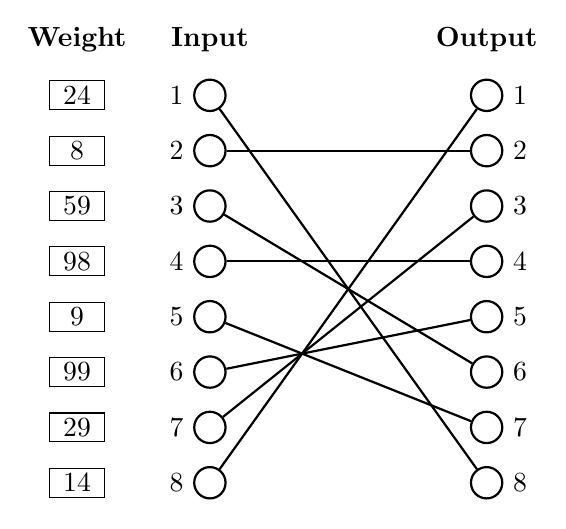
\begin{tikzpicture}[
vertex/.style={circle, draw, inner sep=4pt, thick},
edge/.style={thick},
weight/.style={rectangle, draw, inner sep=2pt, minimum width=20pt},
info/.style={draw=none,fill=none,inner sep=0pt}]

%% local variables
\def \margin{48pt}
\def \hm {100pt}
\def \vm {20pt}
\def \NUMOFVERTICES {8} 

%% place all input vertices
\foreach \s in {1,...,\NUMOFVERTICES}
      \node[vertex,label=left:$\s$] (I-\s) at (0,{- (\s - 1) * \vm}) {};

%% place all output vertices
\foreach \s in {1,...,\NUMOFVERTICES}
      \node[vertex,label=right:$\s$] (O-\s) at (\hm,{- (\s - 1) * \vm}) {};

\node[info] (I) at (0,{- (\NUMOFVERTICES - 1) * \vm}) {};
\node[info] (O) at (\hm,{- (\NUMOFVERTICES - 1) * \vm}) {};

%% place other ifnormation
\node[info] (in) at (0,\vm) {\bf Input};
\node[info] (out) at (\hm, \vm){\bf Output};
\node[info] (weight) at ({-\margin}, \vm) {\bf Weight};

%% matching information
% ==========================================
% 1 8 24
% 2 2 8
% 3 6 59
% 4 4 98
% 5 7 9
% 6 5 99
% 7 3 29
% 8 1 14
% ==========================================

%% place all weight right of output vertices
\node[weight] (W-1) at ({-\margin},{- (0) * \vm}) {$24$};
\node[weight] (W-2) at ({-\margin},{- (1) * \vm}) {$8$};
\node[weight] (W-3) at ({-\margin},{- (2) * \vm}) {$59$};
\node[weight] (W-4) at ({-\margin},{- (3) * \vm}) {$98$};
\node[weight] (W-5) at ({-\margin},{- (4) * \vm}) {$9$};
\node[weight] (W-6) at ({-\margin},{- (5) * \vm}) {$99$};
\node[weight] (W-7) at ({-\margin},{- (6) * \vm}) {$29$};
\node[weight] (W-8) at ({-\margin},{- (7) * \vm}) {$14$};

%% place all edges
\foreach \i/\o in {1/8, 2/2, 3/6, 4/4, 5/7, 6/5, 7/3, 8/1}
      \draw[edge] (I-\i) -- (O-\o);

\end{tikzpicture}
\end{document}